\documentclass[11pt]{article}

% Language setting
% Replace `english' with e.g. `spanish' to change the document language
\usepackage[french]{babel}




% Set page size and margins
% Replace `letterpaper' with `a4paper' for UK/EU standard size
\usepackage[a4paper,top=2cm,bottom=2cm,left=3cm,right=3cm,marginparwidth=1.75cm]{geometry}

% Useful packages
\usepackage{amsmath}
\usepackage{graphicx}
\usepackage[colorlinks=true, allcolors=blue]{hyperref}
\usepackage{minted}
\usepackage{rotating}
\usepackage{tikz}

\title{\bf Le jeu de la vie : rapport de projet}
\author{Joffrey Cottin, Clarine Azinmedem, Christophe Ravier}

\begin{document}

\vfill

{\Huge \maketitle}

\vfill

\newpage

\tableofcontents

\newpage

\section{Des recherches à la première feuille de route}

Nous sommes partis sur l'idée de travailler autour du jeu de la vie, un thème déjà bien étudié mais sur lequel on trouve encore régulièrement des nouvelles découvertes aussi bien mathématiques qu'algorithmiques. Dans le cadre de notre projet, ce choix offre l'avantage de devoir penser les algorithmes aussi bien pour gérer les données "spatiales" (la grille, théoriquement infinie) que "temporelles" (l'évolution, sur un nombre de générations potentiellement très grand) et donc de devoir travailler pour obtenir des algorithmes efficaces. Le sujet permet aussi d'introduire naturellement une interface graphique, tout d'abord pour offrir une visualisation des évolutions de la population au fil des générations mais aussi pour offrir à l'utilisateur des possibilités d'interaction afin de faire ses propres expérimentations (placements dans la grille, sauvegardes ...)

Afin de mieux cerner le sujet et pour réfléchir au contenu à intégrer, nous avons débuté le travail par quelques recherches bibliographiques  autour des automates cellulaires (introduits par Von Neumann alors qu'il travaillait sur des systèmes autoréplicatifs), leur rôle, les questions scientifiques à leur sujet, voire métaphysiques -- certains envisageant l'univers comme un automate cellulaire simple dont les lois physiques seraient des propriétés émergentes ; {\it cf} bibliographie~(page \pageref{biblio}).

À partir de là, une première réflexion à propos du contenu minimal du projet (faire tourner le code du jeu de la vie dans une console Python) a permis d'arriver à une première feuille de route, présentant les étapes vers ce contenu minimal ainsi que ce qui pourrait l'étoffer pour obtenir un projet complet. Le travail en équipe sur la feuille de route a été l'occasion d'apprendre à utiliser Github, ce qui a été bien utile par la suite au moment de partager le code.

Cette feuille de route "idéale" (page \pageref{feuille}) a été utile pour garder à l'esprit les différents objectifs et les hiérarchiser. D'un point de vue de la réalisation pratique, la vie privée et professionnelle (travail à temps plein en dehors du DU) a beaucoup pesé sur les ambitions initiales, générant une importante frustration. Ceci ajouté au fait que, si le travail de groupe est toujours difficile à organiser, il l'est encore plus à distance entre trois personnes qui ne se connaissent pas et ne se croisent jamais. Pour palier aux difficultés de coordinations, nous avons utiliser GitHub est un site web et un service de cloud qui aide les développeurs à stocker et à gérer leur code, ainsi qu’à suivre et contrôler les modifications qui lui sont apportées.

%\newpage 

\section{Le code}

\subsection{Règles du jeu de la vie, version classique de John H. Conway}

Le jeu se déroule sur une grille rectangulaire de cellules ayant un état binaire : elles sont soit vivantes, soit mortes. L'évolution temporelle se fait de façon discrète : le nouvel état de toutes les cellules de la grille est mis à jour simultanément en fonction de leur voisines à l'état précédent. La règle de transition est dite B3/S23 (pour Born 3, Stay 2 ou 3) qui signifie qu'une cellule morte devient vivante si elle possède exactement 3 voisines vivantes et qu'une cellule vivante reste en vie si elle possède 2 ou 3 voisines vivantes. Dans les autres cas, une cellule morte reste morte et une cellule vivante décède.

\begin{figure}[h]
    \centering%    
    % \documentclass[tikz]{standalone}
% \usepackage{tikz}
% \begin{document}

\tikzstyle{morte} = [minimum width= 1cm, minimum height = 1cm, rectangle, fill=blue!65]
\tikzstyle{vivante} = [minimum width= 1cm, minimum height = 1cm, rectangle, fill=red!65]

\begin{tikzpicture}
\node[vivante] at (0,2) {};
\node[morte] at (0,1) {};
\node[vivante] at (0,0) {};
\node[morte] at (1,2) {};
\node[vivante] at (1,1) {};
\node[morte] at (1,0) {};
\node[vivante] at (2,2) {};
\node[morte] at (2,1) {};
\node[morte] at (2,0) {};

\foreach \x in {-0.5,0.5,...,2.5}{
    \draw (\x,-0.5) -- (\x,2.5);
}    
\foreach \y in {-0.5,0.5,...,2.5}{
    \draw (-0.5,\y) -- (2.5,\y);
}

\draw[->,>=stealth] (3,1) -- (4,1);

\node[morte] at (5,2) {};
\node[vivante] at (5,1) {};
\node[morte] at (5,0) {};
\node[vivante] at (6,2) {};
\node[vivante] at (6,1) {};
\node[morte] at (6,0) {};
\node[morte] at (7,2) {};
\node[morte] at (7,1) {};
\node[morte] at (7,0) {};

\foreach \x in {4.5,5.5,...,7.5}{
    \draw (\x,-0.5) -- (\x,2.5);
}    
\foreach \y in {-0.5,0.5,...,2.5}{
    \draw (4.5,\y) -- (7.5,\y);
}

\draw[->,>=stealth] (8,1) -- (9,1);

\node[vivante] at (10,2) {};
\node[vivante] at (10,1) {};
\node[morte] at (10,0) {};
\node[vivante] at (11,2) {};
\node[vivante] at (11,1) {};
\node[morte] at (11,0) {};
\node[morte] at (12,2) {};
\node[morte] at (12,1) {};
\node[morte] at (12,0) {};

\foreach \x in {9.5,10.5,...,12.5}{
    \draw (\x,-0.5) -- (\x,2.5);
}    
\foreach \y in {-0.5,0.5,...,2.5}{
    \draw (9.5,\y) -- (12.5,\y);
}
\end{tikzpicture}

% \end{document}



    \caption{\label{fig:transition}Exemple d'une transition B3/S23 dans une configuration plane.}
\end{figure}

\subsection{Implémentation de la version "Terminal"}

Pour implémenter ce jeu, nous avons construit deux classes, l'une implémentant une cellule et l'autre une grille qui permettra de suivre l'évolution du jeu de la vie sur une succession de générations. Pour tout le projet, c'est la notation matricielle qui est utilisée pour se repérer sur la grille, \mintinline{python}{(i, j)} représente ainsi le numéro de ligne puis le numéro de colonne.

\subsubsection{La classe \mintinline{python}{Cellule}}

La classe \mintinline{python}{Cellule} du fichier \mintinline{python}{cellule.py} contient trois attributs : l'état actuel de la cellule, son état futur et la liste des cellules voisines. La nécessité d'avoir deux attributs pour les états vient du fait que le changement d'état de toutes les cellules d'une grille devant être simultané, on ne peut pas modifier l'état d'une cellule avant de l'avoir utilisé sur ses voisines à venir. 

\begin{figure}[h]
\inputminted[numbersep=2pt,linenos=true,frame=single,bgcolor=black!5,firstline=13,lastline=17]{python}{../code/cellule.py} \vspace*{-0.5cm}
\caption{\label{fig:classeCellule}Le constructeur de la classe \mintinline{python}{Cellule} de la version "Terminal"}
\end{figure}

La méthode \mintinline{python}{calcule_etat_futur()} parcourt la liste des voisins de la cellule et, en fonction du nombre de voisins vivants, modifie l'état futur de la cellule considérée. 

\begin{figure}[h]
\inputminted[numbersep=2pt,linenos=true,frame=single,bgcolor=black!5,firstline=51,lastline=65]{python}{../code/cellule.py} \vspace*{-0.5cm}
\caption{La méthode \mintinline{python}{calcule_etat_futur()} de la version "Terminal"}
\end{figure}

\newpage

Puis c'est la méthode \mintinline{python}{basculer()} qui, appelée en temps voulu, modifie l'état actuel de la cellule.
\begin{figure}[!h]
\inputminted[numbersep=2pt,linenos=true,frame=single,bgcolor=black!5,firstline=39,lastline=41]{python}{../code/cellule.py} \vspace*{-0.5cm}
\caption{La méthode \mintinline{python}{basculer()} de la version "Terminal"}
\end{figure}

\noindent Les autres méthodes de cette classe ne sont pas détaillées ici.\\
La fin de cette classe consiste en une série de tests unitaires afin de s'assurer de la correction des méthodes de la classe.

\subsubsection{La classe \mintinline{python}{Grille}}

La classe \mintinline{python}{Grille} du fichier \mintinline{python}{grille.py} contient quatre attributs : le nombre de lignes (\mintinline{python}{nbLignes}) ; de colonnes (\mintinline{python}{nbColonnes}) ; \mintinline{python}{matrix}, un tableau à deux dimensions contenant des cellules (toutes mortes à la création de la grille) et enfin \mintinline{python}{typeg} qui définit le type de grille (plane ou torique).

\begin{figure}[!h]
\inputminted[numbersep=2pt,linenos=true,frame=single,bgcolor=black!5,firstline=19,lastline=26]{python}{../code/grille.py} \vspace*{-0.5cm}
\caption{Le constructeur de la classe \mintinline{python}{Grille} de la version "Terminal"}
\end{figure}

La méthode \mintinline{python}{remplir_alea(taux)} permet de passer aléatoirement selon un taux moyen donné certaines cellules à l'état vivant et la méthode \mintinline{python}{affecte_voisins()} va construire pour chaque cellule sa liste de voisins.

\begin{figure}[!h]
\inputminted[numbersep=2pt,linenos=true,frame=single,bgcolor=black!5,firstline=91,lastline=99]{python}{../code/grille.py} \vspace*{-0.5cm}
\caption{La méthode \mintinline{python}{remplir_alea(taux)} de la classe \mintinline{python}{Grille}}
\end{figure}


Une fois la grille prête à débuter, le déroulement des générations successives du jeu de la vie se fait en deux étapes, ainsi qu'expliqué plus haut.

La méthode \mintinline{python}{jeu()} parcourt les cellules et calcule pour chacune leur état futur, le résultat étant stocké dans l'attribut correspondant de la cellule. 

\begin{figure}[!h]
\inputminted[numbersep=2pt,linenos=true,frame=single,bgcolor=black!5,firstline=101,lastline=107]{python}{../code/grille.py} \vspace*{-0.5cm}
\caption{La méthode \mintinline{python}{jeu()} de la classe \mintinline{python}{Grille}}
\end{figure}

Dans un second temps, lorsque tous les états futurs ont été calculés, la méthode \mintinline{python}{actualise()} re-parcourt la grille et réalise la bascule pour chaque cellule afin d'obtenir la nouvelle génération.

\begin{figure}[!h]
\inputminted[numbersep=2pt,linenos=true,frame=single,bgcolor=black!5,firstline=109,lastline=115]{python}{../code/grille.py} \vspace*{-0.5cm}
\caption{La méthode \mintinline{python}{actualise()} de la classe \mintinline{python}{Grille}}
\end{figure}

Cette classe se termine comme la précédente avec un jeu de tests unitaires afin de tester les différentes méthodes.

\subsubsection{Le fichier \mintinline{python}{jeuVie_Terminal.py}}

Le fichier est le fichier à exécuter via la commande \mintinline{python}{python3 jeuVie_GUI.py} dans un {\tt Terminal}.

\subsection{Implémentation de l'interface graphique}

On utilise tout d’abord deux classes \mintinline{python}{CelluleFrame} et \mintinline{python}{GrilleFrame} implémentant les versions graphiques des classes \mintinline{python}{Cellule} et \mintinline{python}{Grille} aisément grâce à l'héritage multiple.

La figure suivante représente une capture d'écran de l'interface graphique du jeu de la vie à travers laquelle on peut voir les différentes fonctionnalités implémentées.

\bigskip

La classe \mintinline{python}{CelluleFrame} ajoute simplement des informations de couleur de la case et seule la méthode \mintinline{python}{basculer()} est surchargée. 

\newpage

\begin{figure}[!h]
\inputminted[numbersep=2pt,linenos=true,frame=single,bgcolor=black!5,firstline=14,lastline=24]{python}{../code/celluleFrame.py} \vspace*{-1cm}
\caption{Le constructeur de la classe \mintinline{python}{CelluleFrame}}
\end{figure}

Pour la classe \mintinline{python}{GrilleFrame}, c'est essentiellement l'attribut \mintinline{python}{matrix} qui est modifié car, en plus d'être dessinées et colorées, les cases de la grille doivent pouvoir réagir à l'utilisateur. Cette classe contient aussi trois méthodes correspondant au clic de souris, au survol d'une case ou au contraire lorsque le pointeur quitte une case.

\begin{figure}[!h]
\inputminted[numbersep=2pt,linenos=true,frame=single,bgcolor=black!5,firstline=15,lastline=46]{python}{../code/grilleFrame.py} \vspace*{-1cm}
\caption{Le constructeur de la classe \mintinline{python}{GrilleFrame}}
\end{figure}

\newpage

Le fichier \mintinline{python}{jeuVie_GUI.py} est le fichier principal du programme. C'est lui qui construit la fenêtre d'interface grâce à \mintinline{python}{tkinter}. L'attribut \mintinline{python}{gridFrame} est une instance de la classe \mintinline{python}{GrilleFrame} et les différentes méthodes fonctionnent à peu près toutes sur le même principe : récupérer les données entrées par l'utilisateur et modifier l'attribut \mintinline{python}{gridFrame} pour prendre en compte les v\oe{}ux de l'utilisateur.

Par exemple la méthode \mintinline{python}{alea_init_config()} utilise d'abord \mintinline{python}{get_alea_rate()} pour obtenir le taux entré par l'utilisateur puis l'utilise en argument de la méthode \mintinline{python}{remplir_alea()} sur l'attribut \mintinline{python}{gridFrame}.

\begin{figure}[!h]
\inputminted[numbersep=2pt,linenos=true,frame=single,bgcolor=black!5,firstline=136,lastline=140]{python}{../code/jeuVie_GUI.py} \vspace*{-0.5cm}
\caption{La méthode \mintinline{python}{alea_init_config}}
\end{figure}

L'interface graphique réalisée dans ce projet met à la disposition de l'utilisateur un certain nombre de fonctionnalités énumérées ci-après :

\begin{figure}[!h]
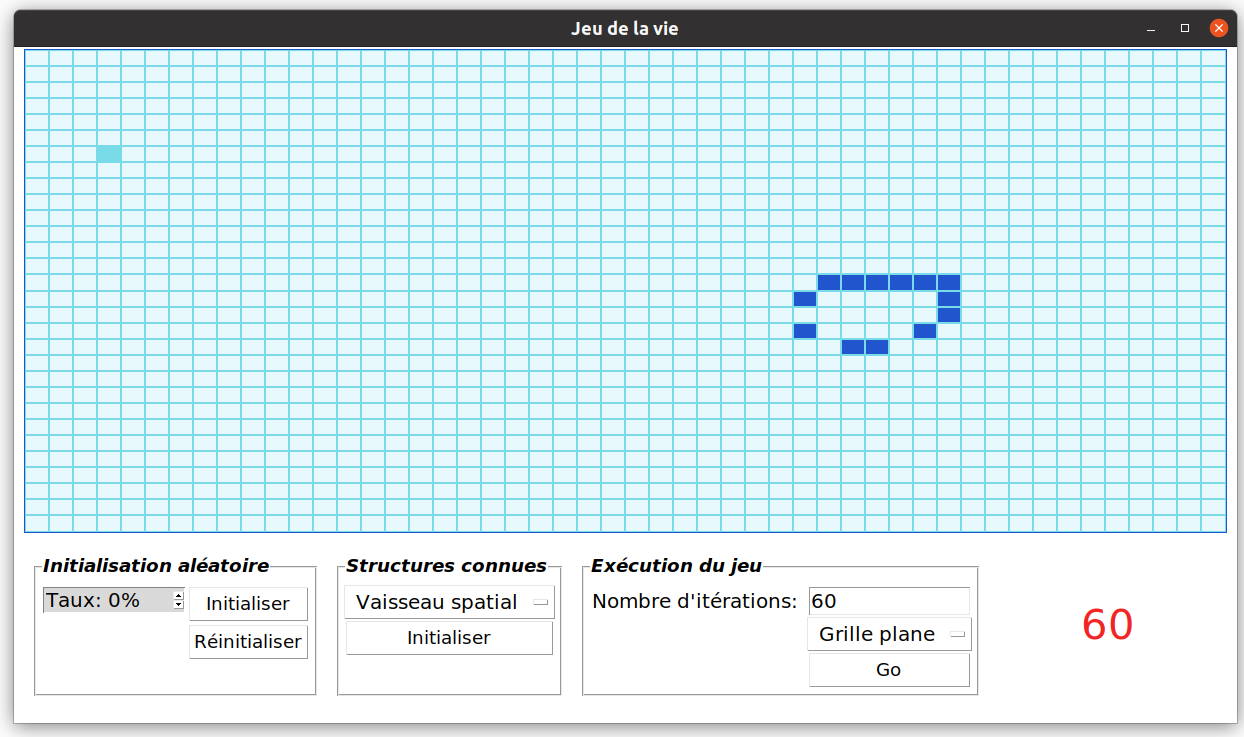
\includegraphics[width=\linewidth]{./images/jdv_exemple.png} \vspace*{-0.5cm}
\caption{Capture d'écran de l'interface graphique}
\end{figure}

\begin{itemize}
    \item {\bf Initialisation aléatoire} : le menu défilant {\it Taux} (instance de la classe \mintinline{python}{ttk.Spinbox}) permet à l'utilisateur de fixer le pourcentage de cellules qui seront vivantes dans la configuration initiale. Une fois le taux fixé, l'utilisateur devra cliquer sur \mintinline{python}{Initialiser} (instance de la classe \mintinline{python}{ttk.Button}) appelant ainsi la méthode \mintinline{python}{alea_init_config()} qui initialise la grille avec le taux choisi. Il est également possible de réinitialiser la grille à travers un click sur le boutton \mintinline{python}{Réinitialiser} qui fait appel à la méthode \mintinline{python}{Reset_grid()}.
    \item {\bf Structures connues} : ici, un menu déroulant (instance de la classe \mintinline{python}{ttk.OptionMenu}) permet à l'utilisateur de choisir une des neuf structures que nous avons mis à sa disposition. Le bouton \mintinline{python}{Initialiser} permet ici d'obtenir une grille avec la configuration de base de la structure choisie.
    \item {\bf Configuration manuelle} : en cliquant sur une cellule quelconque, l'utilisateur peut la rendre vivante ou morte (faisant ainsi appel à la méthode \mintinline{python}{on_cell_click()} de la classe \mintinline{python}{GrilleFrame}).
    Cette fonctionnalité peut par conséquent lui permettre de créer manuellement sa propre configuration initiale.
    \item {\bf Exécution du jeu} : après avoir crée une configuration initiale à l'aide des fonctionnalités énumérées précédemment, l'utilisateur à la possibilité d'insérer dans le champ de texte nombre d'itérations (instance de la classe \mintinline{python}{ttk.Entry}) le nombre de génération à simuler. Il peut également choisir le type de grille (plane ou torique) et ensuite cliquer sur le bouton \mintinline{python}{Go} pour lancer la simulation. La géneration courante est en permanence visible en rouge sur l'écran en bas à droite.
\end{itemize}


\section{Et après?}

Comme déjà mentionné, le manque de temps nous a amené à restreindre nos ambitions et à laisser de côté certaines idées initialement envisagées pour y revenir plus tard, une fois les examens passés par exemple. Parmi les pistes d'amélioration, agrandir la bibliothèque d'exemples (pourquoi pas un canon générateur de nombres premiers ?) et permettre à l'utilisateur de sauvegarder des configurations sous forme d'images. Un peu plus long à implémenter, offrir la possibilité de définir des règles du jeu différentes (en terme d'apparition et de mort des cellules en fonction du voisinage, voire en utilisant un voisinage différent comme celui de Von Neumann) pour étudier des variantes du jeu de la vie. 
A plus long terme, envisager d'autres variantes avec un nombre d'états des cellules différent (exemple du jeu de la vie quantique mentionné dans la bibliographie), et du point de vue algorithmique réfléchir à un programme de reconnaissance de motifs (permettant par exemple d'identifier des configurations stables ou périodiques dans une grille donnée), ou de recherche d'antécédents (travailler sur les jardins d'Eden) et enfin, essayer de comprendre et d'implémenter une version de l'algorithme Hashlife qui a permis dans les années 1980 de grands progrès sur le sujet grâce à des calculs extrêmement efficaces (mais qui dépasse largement le niveau licence!).

\newpage

\section*{ANNEXE\label{feuille} : La feuille de route "idéale"}

\begin{figure}[h]
    \centering%
    \begin{sideways}        
        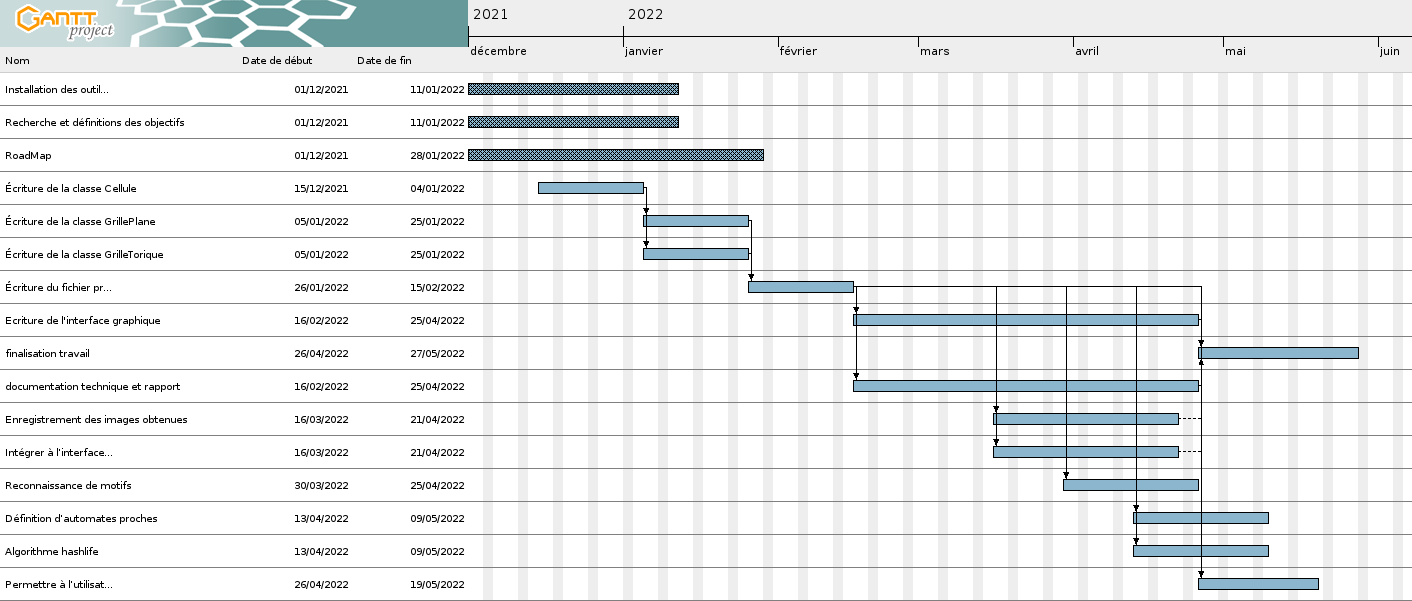
\includegraphics[width=18cm]{./images/roadmap.png}
    \end{sideways}
    \caption{\label{fig:roadmap}la feuille de route.}
\end{figure}

\newpage 

\label{biblio}
\nocite{*}
\bibliographystyle{unsrt}
\bibliography{biblio}

\end{document}
